%
% symmetrien.tex -- Symmetrien
%
% (c) 2021 Prof Dr Andreas Müller, OST Ostschweizer Fachhochschule
%
\bgroup
\definecolor{darkgreen}{rgb}{0,0.6,0}
\begin{frame}[t]
\setlength{\abovedisplayskip}{5pt}
\setlength{\belowdisplayskip}{5pt}
\frametitle{Symmetrien}
\vspace{-20pt}
\begin{columns}[t,onlytextwidth]
\begin{column}{0.48\textwidth}
\begin{block}{Diskrete Symmetrien}
\begin{itemize}
\item<2->
Ebenen-Spiegelung:
\[
{\tiny
\begin{pmatrix*}[r] x_1\\x_2\\x_3 \end{pmatrix*}
}
\mapsto
{\tiny
\begin{pmatrix*}[r]-x_1\\x_2\\x_3 \end{pmatrix*}
}
\uncover<4->{\!,\;
\vec{x}
\mapsto
\vec{x} -2 (\vec{n}\cdot\vec{x}) \vec{n}
}
\]
\vspace{-10pt}
\begin{center}
\begin{tikzpicture}[>=latex,thick]
\def\a{10}
\def\b{50}
\def\r{2}
\coordinate (O) at (0,0);
\coordinate (A) at (\b:\r);
\coordinate (B) at ({180+2*\a-\b}:\r);
\coordinate (C) at ({90+\a}:{\r*cos(90+\a-\b)});
\coordinate (N) at (\a:2);
\coordinate (D) at (\a:{\r*cos(\b-\a)});
\uncover<3->{
\clip (-2.5,-0.45) rectangle (2.5,1.95);

	\fill[color=darkgreen!20] (O) -- ({\a-90}:0.2) arc ({\a-90}:\a:0.2)
		-- cycle;
	\draw[->,color=darkgreen] (O) -- (N);
	\node[color=darkgreen] at (N) [above] {$\vec{n}$};


	\fill[color=blue!20] (C) -- ($(C)+(\a:0.2)$) arc (\a:{90+\a}:0.2)
		-- cycle;
	\fill[color=red] (O) circle[radius=0.06];
	\draw[color=red] ({\a-90}:2) -- ({\a+90}:2);
	\fill[color=blue] (C) circle[radius=0.06];
	\draw[color=blue,line width=0.1pt] (A) -- (D);
	\node[color=darkgreen] at (D) [below,rotate=\a]
		{$(\vec{n}\cdot\vec{x})\vec{n}$};
	\draw[color=blue,line width=0.5pt] (A)--(B);

	\node[color=blue] at (A) [above right] {$\vec{x}$};
	\node[color=blue] at (B) [above left] {$\vec{x}'$};

	\node[color=red] at (O) [below left] {$O$};

	\draw[->,color=blue,shorten <= 0.06cm,line width=1.4pt] (O) -- (A);
	\draw[->,color=blue,shorten <= 0.06cm,line width=1.4pt] (O) -- (B);
}

\end{tikzpicture}
\end{center}
\vspace{-5pt}
$\vec{n}$ ein Einheitsnormalenvektor auf der Ebene, $|\vec{n}|=1$
\item<5->
Punkt-Spiegelung:
\[
{\tiny
\begin{pmatrix*}[r] x_1\\x_2\\x_3 \end{pmatrix*}
}
\mapsto
-
{\tiny
\begin{pmatrix*}[r]x_1\\x_2\\x_3 \end{pmatrix*}
}
\]
\end{itemize}
\end{block}
\end{column}
\begin{column}{0.48\textwidth}
\uncover<6->{%
\begin{block}{Kontinuierliche Symmetrien}
\begin{itemize}
\item<7-> Translation:
\(
\vec{x} \mapsto \vec{x} + \vec{t}
\)
\item<8-> Drehung:
\vspace{-3pt}
\begin{center}
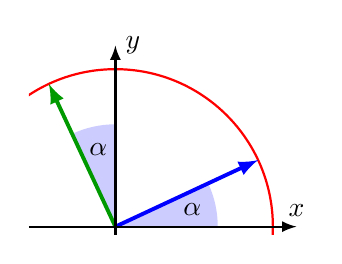
\begin{tikzpicture}[>=latex,thick]
\def\a{25}
\def\r{1.3}
\coordinate (O) at (0,0);
\begin{scope}
\clip (-1.1,-0.1) rectangle (2.3,2.3);
\draw[color=red] (O) circle[radius=2];
\fill[color=blue!20] (O) -- (0:\r) arc (0:\a:\r) -- cycle;
\fill[color=blue!20] (O) -- (90:\r) arc (90:{90+\a}:\r) -- cycle;
\node at ({0.5*\a}:1) {$\alpha$};
\node at ({90+0.5*\a}:1) {$\alpha$};
\draw[->,color=blue,line width=1.4pt] (O) -- (\a:2);
\draw[->,color=darkgreen,line width=1.4pt] (O) -- ({90+\a}:2);
\end{scope}
\draw[->] (-1.1,0) -- (2.3,0) coordinate[label={$x$}];
\draw[->] (0,-0.1) -- (0,2.3) coordinate[label={right:$y$}];
\end{tikzpicture}
\end{center}
\[
\uncover<9->{%
\begin{pmatrix}x\\y\end{pmatrix}
\mapsto
\begin{pmatrix}
{\color{blue}\cos\alpha}&{\color{darkgreen}-\sin\alpha}\\
{\color{blue}\sin\alpha}&{\color{darkgreen}\phantom{-}\cos\alpha}
\end{pmatrix}
\begin{pmatrix}x\\y\end{pmatrix}
}
\]
\end{itemize}
\end{block}}
\vspace{-10pt}
\uncover<10->{%
\begin{block}{Definition}
Längen/Winkel bleiben erhalten
\\
\uncover<11->{%
$\Rightarrow$ $\exists$ Erhaltungsgrösse}
\end{block}}
\end{column}
\end{columns}
\end{frame}
\egroup
